\input format.tex

\usepackage{graphicx}
\graphicspath{{cores/}}

\usepackage{environ}
\usepackage{colortbl,array,booktabs}
\usepackage{tabularx}

\colorlet{TablaBordeSuperior}{topcolor}
\colorlet{TablaBordeInferior}{topcolor}
\colorlet{TablaCentroSuperior}{blue!1}
\colorlet{TablaCentroInferior}{blue!20}
\colorlet{FuenteCabeceraTabla}{white}

\newcolumntype{M}[1]{>{\centering\arraybackslash}m{#1}}
%\newcommand{\tabularxcolumn}[1]{>\arraybackslash}m{#1}}

\tcbset{rtab/.style={
freelance,
frame code={
 \path[top color=topcolor,bottom color=topcolor]
   ([yshift=-#1*(\baselineskip+2pt)]interior.north west) --
   ([yshift=-#1*(\baselineskip+2pt)]interior.north east) {[sharp corners]--
    ([yshift=3pt]interior.north east) --
    ([yshift=3pt]interior.north west)} -- cycle;

  },
interior code={},
 }
}

\newcommand\fuentecabecera[1]{\textcolor{black}{\textbf{#1}}}

\begin{document}

\vspace*{4mm}
%% 各章节
\setlength{\arrayrulewidth}{.2pt}
\fontsize{8.8pt}{11pt}\selectfont
\color{gray2}

\begin{center}
{\noindent\bf\sanhao 二、检测结果解析}
\end{center}

\vspace*{3mm}

\noindent{\bf{肠道微生态平衡能力}}

\begin{spacing}{1.5}

\begin{LRaside}[.8]{\fontsize{8.8pt}{11pt}\selectfont 检测说明}
\noindent
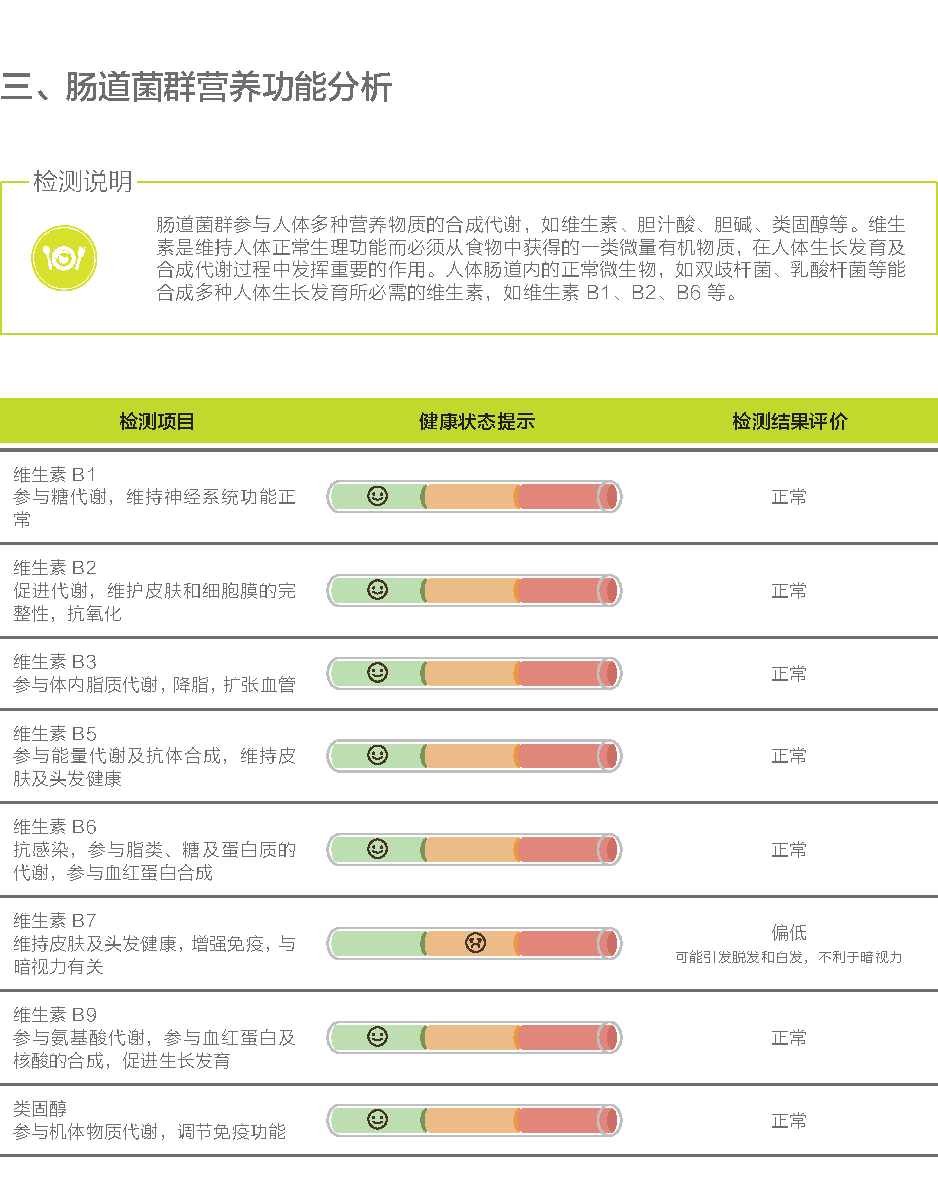
\includegraphics[width=\linewidth]{yingyanggongneng.pdf}
\asidebreak %
{\fontsize{8pt}{11pt}\selectfont 人体肠道内存在上万亿个细菌,不同菌群共同组成了复杂的肠道微生态系统。国际最新权威研究重新定义肥胖,发现肠道菌群与肥胖关系密切,肠道微生态失衡极易引起肥
胖。肠道微生态平衡能力越高,肠道微生态越稳定,发生肥胖的风险越低;肠道微生态平衡能力越低,肠道微生态容易失调,易引发肥胖等健康问题。而肠道菌群结构中的有益菌
能保护肠道微生态结构,防止其被破坏;而有害菌可破坏肠道微生态结构,当微生态失衡,有害菌异常增殖,易引发肥胖等。因此,通过检测发现导致肠道微生态失衡的已有或
潜在因素,有效减重或预防肥胖的发生。}
\end{LRaside}

\end{spacing}

\noindent 检测结果

\hfill {\bf {肠道微生态平衡能力 \quad}
{\color{green4}好}
}

\begin{tctabularx}{tabularx={m{4cm}<{\centering}m{6.6cm}<{\centering}m{4cm}<{\centering}}}
&&
\\[-6pt]
\cellcolor{topcolor} \raisebox{2.614pt}{\color{gray2}\bf 检测项目} &
\cellcolor{topcolor} \raisebox{2.614pt}{\color{gray2}\bf 健康状态提示} &
\cellcolor{topcolor} \raisebox{2.614pt}{\color{gray2}\bf 检测结果评价}
\end{tctabularx}

\vspace*{-4.25mm}
\fontsize{8pt}{11pt}\selectfont
\arrayrulecolor{gray2}
\begin{longtable}{m{4cm}<{\centering}m{6.6cm}<{\centering}m{0cm}@{}m{4cm}<{\centering}}
\hline
\parbox[c]{\hsize}{\vskip7pt {\lantxh 肠道菌群多样性} \vskip7pt} & \parbox[c]{\hsize}{\vskip7pt\centerline{\raisebox{-1.5ex}{
\includegraphics[width=6cm,height=0.55cm]{bar01.pdf}}}\vskip7pt}  &
\hspace*{-5.08cm}\raisebox{-0.75ex}{
\includegraphics{cry.pdf}}
 & \begin{minipage}{4cm}\begin{center}{{\lantxh 偏低} }\end{center} \end{minipage} \\
\hline
\parbox[c]{\hsize}{\vskip7pt {\lantxh 有益菌} \vskip7pt} & \parbox[c]{\hsize}{\vskip7pt\centerline{\raisebox{-1.5ex}{
\includegraphics[width=6cm,height=0.55cm]{bar01.pdf}}}\vskip7pt}  &
\hspace*{-5.08cm}\raisebox{-0.75ex}{
\includegraphics{cry.pdf}}
 & \begin{minipage}{4cm}\begin{center}{{\lantxh 偏低} }\end{center} \end{minipage} \\
\hline
\parbox[c]{\hsize}{\vskip7pt {\lantxh 有害菌} \vskip7pt} & \parbox[c]{\hsize}{\vskip7pt\centerline{\raisebox{-1.5ex}{
\includegraphics[width=6cm,height=0.55cm]{bar02.pdf}}}\vskip7pt}  &
\hspace*{-5.08cm}\raisebox{-0.75ex}{
\includegraphics{smile.pdf}}
 & \begin{minipage}{4cm}\begin{center}{{\lantxh 偏低} }\end{center} \end{minipage} \\
\hline

\parbox[c]{\hsize}{{\lantxh 致病菌}}
& \parbox[c]{\hsize}{\vskip7pt \centering{\lantxh 小韦荣氏球菌} \vskip7pt} & & \begin{minipage}{4cm}\begin{center}{{\lantxh 超标} }\end{center} \end{minipage} \\\cline{2-4}
\hline
\end{longtable}

\vspace*{3mm}

\begin{spacing}{1.5}

\begin{LRaside}[.8]{\fontsize{8.8pt}{11pt}\selectfont 结果分析}
\noindent

\includegraphics[width=\linewidth]{result_fenbu.pdf}
\asidebreak %
\fontsize{8pt}{11pt}\selectfont
您的肠道菌群微生态平衡能力
非常好,菌群失衡风险低,有利于肠道健康,不会增加减重难度。
但其中肠道菌群多样性、有益菌指标异常,仍需及时调理肠道菌群,提高肠道微生态平衡能力。

\noindent 另外致病菌小韦荣氏球菌含量超标,易引起腹胀腹泻等肠道不适症状,需密切关注,请定期复查。

\end{LRaside}

\end{spacing}

\end{document}

